\section{Phần 3 -- Localization với bản đồ đã lưu}

\subsection{Quy trình}
Sau khi lưu bản đồ: dừng SLAM Toolbox, chạy \code{kill\_sim.sh} rồi \code{start\_sim.sh} + \code{unlock\_robot.sh} để khởi động lại robot trong cùng world,
sau đó chạy:
\begin{lstlisting}[language=bash,caption={\file{scripts/start\_localization.sh}.}]
exec ros2 launch turtlebot4_navigation localization.launch.py use_sim_time:=true \
  map:="$DIR/maps/map.yaml" params:="$DIR/config/localization.yaml" "$@"
\end{lstlisting}
Launch này gọi \code{nav2\_bringup/localization\_launch.py}, khởi động \code{map\_server} (nạp \file{maps/map.yaml}, phát \code{/map})
và \code{amcl}, được quản lý bởi \code{lifecycle\_manager\_localization}. Log xác nhận cả hai node ở trạng thái \emph{active}:
\begin{lstlisting}[numbers=none,basicstyle=\ttfamily\footnotesize,caption={Log \code{start\_localization.sh} (rút gọn).}]
[lifecycle_manager_localization]: Server amcl connected with bond.
[lifecycle_manager_localization]: Managed nodes are active
[amcl]: AMCL cannot publish a pose or update the transform. Please set the initial pose...
\end{lstlisting}
Dòng cuối là bình thường: AMCL cần vị trí ban đầu mới bắt đầu phát \code{/amcl\_pose}.

\subsection{Tham số AMCL (\file{config/localization.yaml})}
Giữ nguyên cấu hình của \code{turtlebot4\_navigation}: mô hình chuyển động vi sai (\code{DifferentialMotionModel}), mô hình cảm biến
\code{likelihood\_field}, \code{min\_particles}=500, \code{max\_particles}=2000, \code{update\_min\_d}=0,25\,m, \code{update\_min\_a}=0,2\,rad,
\code{global\_frame\_id: map}, \code{odom\_frame\_id: odom}, \code{base\_frame\_id: base\_link}, \code{tf\_broadcast: true}.
Nghĩa là AMCL chỉ cập nhật khi robot đi quá 0,25\,m hoặc quay quá 0,2\,rad, và bù lệch bằng cách phát TF \code{map}$\to$\code{odom}.

\subsection{Đặt vị trí ban đầu}
AMCL cần \code{/initialpose} (tương đương công cụ \emph{2D Pose Estimate} trong RViz2). Em dùng script publish \code{PoseWithCovarianceStamped}:
\begin{lstlisting}[language=Python,caption={Trích \file{scripts/set\_initial\_pose.py}.}]
msg.header.frame_id = 'map'
msg.pose.pose.position.x = x
msg.pose.pose.position.y = y
msg.pose.pose.orientation.z = math.sin(yaw / 2.0)
msg.pose.pose.orientation.w = math.cos(yaw / 2.0)
cov[0] = cov[7] = sxy ** 2      # phuong sai vi tri (mac dinh sigma 0.5 m)
cov[35] = syaw ** 2             # phuong sai huong (mac dinh sigma 0.26 rad ~ 15 do)
\end{lstlisting}
Hiệp phương sai càng nhỏ thì các hạt (particle) càng tập trung quanh vị trí cung cấp.

Vì Gazebo ở máy này không cung cấp được vị trí thật (topic \code{/sim\_ground\_truth\_pose} xung đột QoS), em tự tìm vị trí robot từ bản đồ bằng
\file{scripts/find\_pose.py}: lấy một bản tin \code{/scan}, thử lưới các tư thế $(x,y,\theta)$ trên bản đồ và chọn tư thế làm các điểm scan rơi sát tường nhất
(sai số RMS đến ô tường gần nhất, dùng distance transform):
\begin{lstlisting}[language=Python,caption={Trích \file{scripts/find\_pose.py}.}]
gx, gy = x + c * lx - sn * ly, y + sn * lx + c * ly      # diem scan -> frame map
ix = ((gx - OX) / RES).astype(int);  iy = H - 1 - ((gy - OY) / RES).astype(int)
e = np.sqrt(np.mean(dist[iy[m], ix[m]] ** 2))            # RMS khoang cach toi tuong gan nhat
\end{lstlisting}

\subsection{Kết quả}
\begin{lstlisting}[numbers=none,basicstyle=\ttfamily\footnotesize,caption={Đặt initial pose và kiểm tra AMCL (\file{scripts/check\_localization.py}).}]
$ python3 scripts/find_pose.py -0.8 0.4 -0.6 0.4
best -0.10 -0.17 2.862 ...                      # x, y, yaw(rad) khop voi ban do
$ python3 scripts/set_initial_pose.py -0.10 -0.17 2.862 0.15 0.15
Da dat initial pose: x=-0.1 y=-0.17 yaw=2.862 rad (frame map)
[amcl]: Setting pose: -0.100 -0.170 2.862
$ python3 scripts/check_localization.py
AMCL  : x=-0.089 y=-0.174 yaw=164.1 deg
        do bat dinh: sigma_x=0.155 m  sigma_y=0.152 m  sigma_yaw=8.3 deg
\end{lstlisting}
AMCL báo $(-0{,}089;\,-0{,}174;\,164{,}1^\circ)$, trùng với kết quả khớp scan--bản đồ $(-0{,}10;\,-0{,}17;\,164{,}0^\circ)$, độ bất định còn khoảng
15\,cm và $8^\circ$. Cần lưu ý đây \textbf{không phải một phép kiểm chứng độc lập}, vì chính kết quả khớp scan đã được dùng làm initial pose;
nó chỉ cho thấy AMCL giữ được tư thế đó. Kiểm chứng thực tế là: tia LiDAR trong RViz2 phải trùng các tường của bản đồ và đám hạt phải tụ gọn
quanh robot (hình bên dưới), và trong Phần 4 robot đi đến đúng các điểm trên bản đồ.

\paragraph{Lưu ý khi đặt initial pose.} Các lần đầu em đặt initial pose theo ước lượng bằng mắt (ví dụ $(0,0,0)$ hoặc theo \code{/odom}). Sau khi robot di chuyển,
AMCL vẫn ở tư thế lệch: tại một thời điểm, tư thế AMCL cho sai số khớp scan--bản đồ 0,34\,m, trong khi tư thế tìm bằng \code{find\_pose.py} chỉ 0,09\,m.
AMCL chỉ cập nhật khi robot đi đủ xa và cần initial pose đủ gần mới hội tụ đúng, nên em chuyển sang dùng \code{find\_pose.py} để lấy initial pose.
Em chưa xác định chắc nguyên nhân gốc của sai lệch ban đầu (nghi do vị trí/hướng robot sau undock khác giả định, và sim chạy chậm làm TF đến trễ).

\anh[0.7]{fig_map_loaded.png}{RViz2 sau khi \code{map\_server} nạp lại \file{maps/map.yaml}: bản đồ đã lưu hiện lên trên topic \code{/map} (chưa đặt initial pose nên chưa có robot trên bản đồ).}
\begin{figure}[H]\centering
\begin{subfigure}{0.49\linewidth}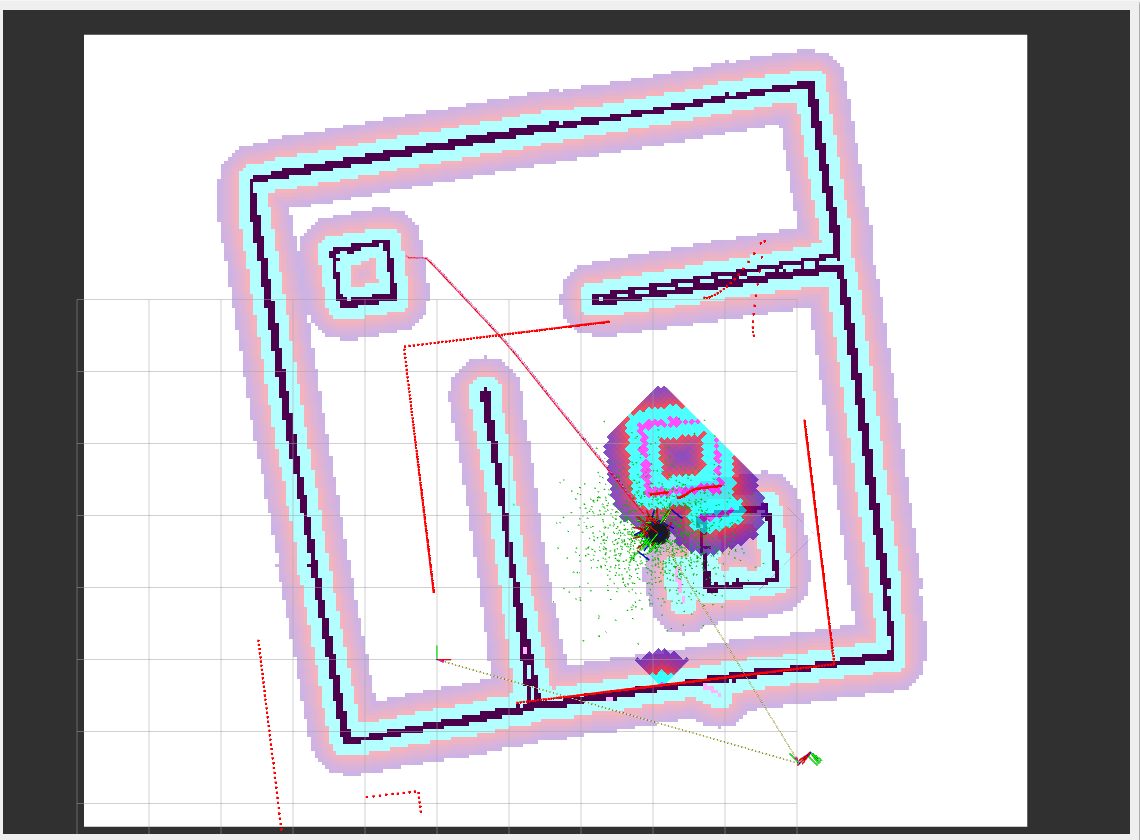
\includegraphics[width=\linewidth]{fig_amcl_before.png}\caption{initial pose với $\sigma_{xy}=0{,}5$\,m, $\sigma_\theta=0{,}4$\,rad: hạt (chấm xanh lá) rải rộng.}\end{subfigure}\hfill
\begin{subfigure}{0.49\linewidth}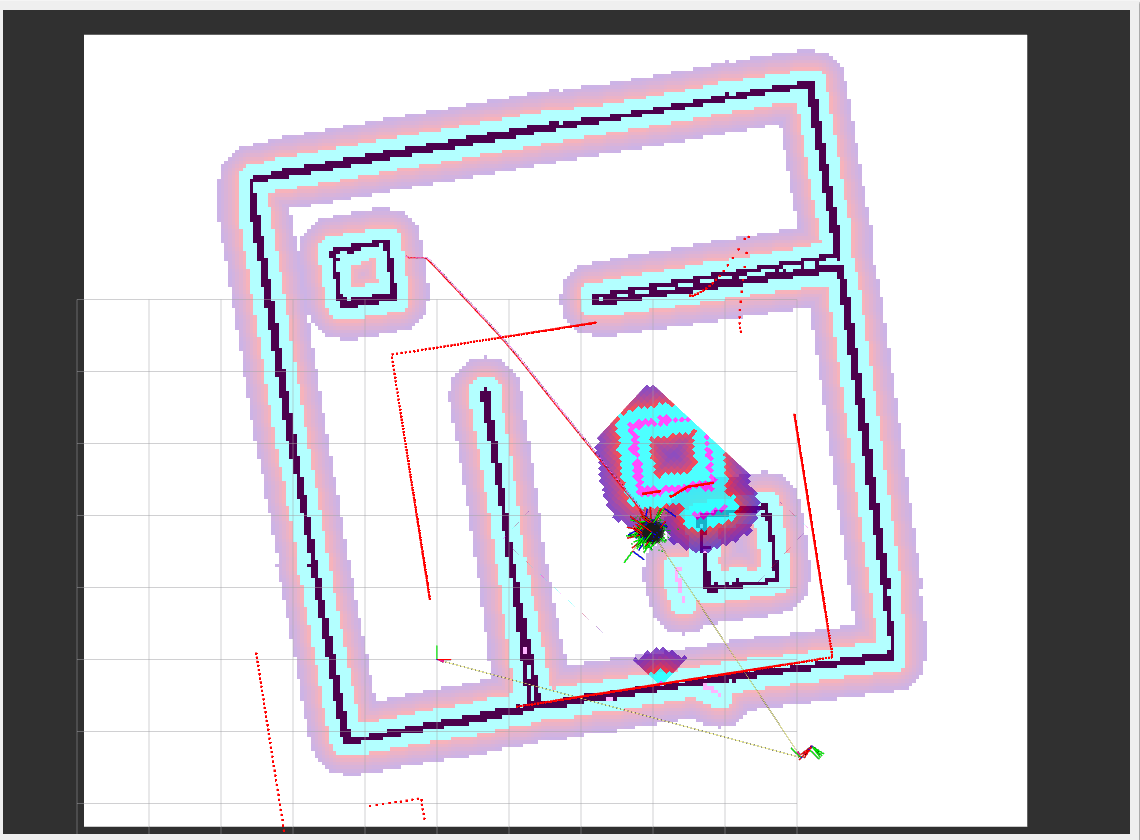
\includegraphics[width=\linewidth]{fig_amcl_after.png}\caption{với $\sigma_{xy}=0{,}1$\,m, $\sigma_\theta=0{,}1$\,rad: hạt tụ gọn quanh robot; AMCL báo $\sigma\approx0{,}10$\,m, $5{,}4^\circ$.}\end{subfigure}
\caption{Đám hạt AMCL trong RViz2 (vùng màu quanh robot là local costmap; tia LiDAR đỏ trùng tường bản đồ).}\end{figure}
